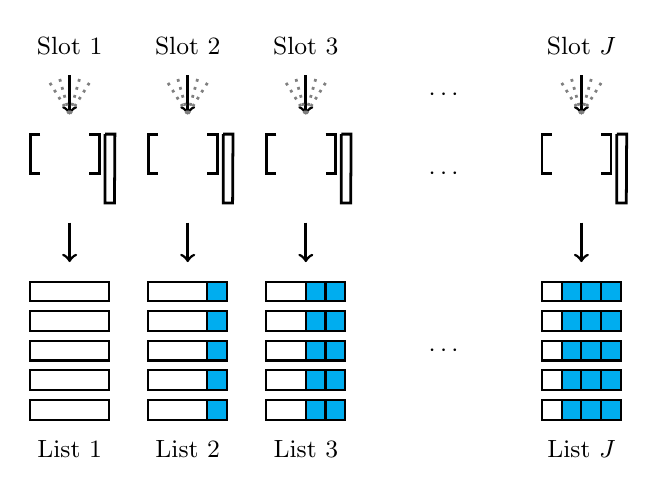
\begin{tikzpicture}
[font=\small, draw=black, line width=0.75pt,
sub0/.style={rectangle, draw, inner sep=0pt, minimum width=10mm, minimum height=2.5mm},
parity/.style={rectangle, draw, fill=cyan, inner sep=0pt, minimum size=2.5mm}]

\node (cs1) at (-1.00,6.125) {Slot~1};
\node (cs2) at (0.50,6.125) {Slot~2};
\node (cs3) at (2.00,6.125) {Slot~3};
\node (cs4) at (5.50,6.125) {Slot~$J$};

\foreach \v in {-1.00,0.50,2.00,5.50} {
  \draw[->, line width=1pt]  (\v,3.875) -- (\v,3.375);
  \draw[->, line width=1pt]  (\v,5.75) -- (\v,5.25);
  \draw[dotted, line width=1pt, draw=gray]  (\v-0.25,5.65) -- (\v,5.25);
  \draw[dotted, line width=1pt, draw=gray]  (\v-0.125,5.7) -- (\v,5.25);
  \draw[dotted, line width=1pt, draw=gray]  (\v+0.125,5.7) -- (\v,5.25);
  \draw[dotted, line width=1pt, draw=gray]  (\v+0.25,5.65) -- (\v,5.25);
}

\node (dots1) at (3.75,5.5) {$\cdots$};

\foreach \v in {-1.00,0.50,2.00,5.50} {
  \draw[line width=1pt] (\v-0.375,5) -- (\v-0.5,5) -- (\v-0.5,4.5) -- (\v-0.375,4.5);
  \draw[line width=1pt] (\v+0.25,5) -- (\v+0.375,5) -- (\v+0.375,4.5) -- (\v+0.25,4.5);
  \draw[line width=1pt] (\v+0.45,5) -- (\v+0.45,4.125) -- (\v+0.57,4.125) -- (\v+0.575,5) -- (\v+0.45,5);
}

\node (dots2) at (3.75,4.5) {$\cdots$};
\node (dots3) at (3.75,2.25) {$\cdots$};

\foreach \c in {3.00, 2.625, 2.25, 1.875, 1.5} {
  \node[sub0] (subcs0\c) at (-1.00,\c) {};
  \node[sub0] (subcs2\c) at (0.50,\c) {};
  \node[parity] (parity0\c) at (0.875,\c) {};
  \node[sub0] (subcs3\c) at (2.00,\c) {};
  \node[parity] (parity1\c) at (2.125,\c) {};
  \node[parity] (parity2\c) at (2.375,\c) {};
  \node[sub0] (subcsz\c) at (5.50,\c) {};
  \node[parity] (parity3\c) at (5.375,\c) {};
  \node[parity] (parity4\c) at (5.625,\c) {};
  \node[parity] (parity5\c) at (5.875,\c) {};
}

\node (list1) at (-1.00,1) {List~1};
\node (list2) at (0.50,1) {List~2};
\node (list3) at (2.00,1) {List~3};
\node (list4) at (5.50,1) {List~$J$};
\end{tikzpicture}
